


\chapter{Transport mésoscopique}


Dans ce chapitre nous allons aborder le transport à travers une structure nanoscopique et nous allons nous intéresser en particulier au phénomène de blocage de Coulomb. Ce phénomène a d'abord été observé sur des échantillon métallique macroscopique composé de petit grain métallique par C.J. Gorter en 1951. En mesurant la conductance d'un de ces échantillon en fonction de la température, l'auteur a constaté une diminution inattendu à basse température. Cette diminution de la température à été attribué à l'aspect granuleux du métal. Plus précisément , pour ajouter un électron dans un des grains constituant le métal, il fallait fournir une énergie $e^2/C$ où $e$ est la charge de l'électron et $C$ est la capacité que l'on peut associé à un de ces grains. A haute température ($k_bT \gg e^2/C$), cette énergie n'affecte pas la conductance du système. A basse température en revanche ($k_bT \ll e^2/C$), cette enérgie réduit l'habilité des électron à se mouvoir librement dans le métal ce qui entraîne une diminution de la conductance. Depuis, l'étude de ce phénomène à beaucoup évolué et de nos jours et le rôle central du grain de métal est souvent remplacé par des molécules, des point quantique de gaz d'électron à deux dimensions etc..

Dans ce chapitre, nous verrons tout d'abord qu'elles sont le différent paramètres physique d'un système type. En particulier, nous donnerons quelques conditions nécessaire à l'apparition d'un phénomène de blocage de Coulomb classique et quantique. Nous aborderons ensuite la notion de potentiel chimique et nous montrerons comment cette notion peut expliquer de façon intuitive le phénomène de blocage de Coulomb. Nous déterminerons notamment comment certain paramètre du système par une simple mesure de courant. Nous développerons ensuite un modèle plus quantitatif afin de déterminer le courant circulant à travers une structure nanoscopique. Pour cela, nous nous concentrerons sur le cas particulier d'une boite quantique oscillant entre deux états de charge.
%%%%%%%%%%%%%%%%%%%%%%%%
%SECTION I
%%%%%%%%%%%%%%%%%%%%%%%%


\section{Les paramètres du système}
Dans la suite de ce chapitre, nous considérerons un système simple composé d'un point quantique~(ou ilôt) connecté à trois terminaux que l'on nommera source, drain et grille. L'il\^ot est couplé à ces trois terminaux par trois capacitances : $C_g$ pour la grille, $C_d$ pour le drain et $C_s$ pour la source. De plus, des barrière tunnel entre le point quantique et la source et le drain permettent le passage d'électron (sous certaines conditions). Ces deux barrières tunnels sont caractérisées par les paramètre $\gamma_s$ pour le système source/il\^ot et $\gamma_d$ pour le système drain/il\^ot. La source et le drain sont considérés comme des matériaux métalliques massifs et dont les électrons obéissent à la statistique de Fermi-Dirac. Enfin, nous attribuons à l'il\^ot une taille caractéristique $L$. 

Ce système, les paramètres qui le caractérisent ainsi qu'un schéma électrique équivalent sont représentés dans la Fig. \ref{description_systeme}. Nous allons maintenant détailler chacun de ces éléments de façon plus précise.


\subsection{Les capacitances du système}
Comme expliqué précédemment, trois capacitances couples l'il\^ot central aux trois terminaux. L'application d'un tension sur l'un ou plusieurs terminaux va donc modifier l'energie des électrons situés sur le point quantique. Cette modification peut facilement s'exprimer comme suit :

\begin{eqnarray}
E = \frac{(C_sV_s + C_dV_d + C_gV_g)^2}{2(C_g + C_s + C_g)}=\frac{(C_sV_s + C_dV_d + C_gV_g)^2}{2C_{\Sigma}} \nonumber
\end{eqnarray}

C'est la possibilité de moduler continuement cette énergie qui permet d'effectuer une spectroscopie des états énergétiques comme nous le verrons dans la suite. Il est à noté que dans les expériences de Microscopie à Effet Tunnel ou Scanning Tunneling Microscopie~(STM), seul les tensions de source et de drain peuvent \^etre modifiées. L'équivalent de la tension de grille est joué par l'environement électrostatique et hors d'accès pour l'expérimentateur. Ce désavantage est compensé par la possibilité de modifier les paramètres de couplage $\gamma$~(que l'on détaillera dans la suite) en modulant la distance séparant la pointe de l'échantillon.

Ces capacitance vont également induire un "co\^ut" énergétique à l'ajout d'un électron dans l'il\^ot central. Cet ajout est associé à l'énergie $\frac{E_c}{2}$ appelé énergie de charge~(nous verrons l'utilité du facteur un-demi dans la suite ) dont la valeur est donnée par :
\begin{eqnarray}
\frac{E_c}{2} = \frac{e^2}{2(C_s+C_d+C_g)}=\frac{e^2}{2C_{\Sigma}} \nonumber
\end{eqnarray}


Cette énergie est à l'origine de la diminution de la conductance observée par C.J. Gorter en 1951. Lorsque la température est suffisamment élevée, elle fourni l'énergie nécessaire aux électrons pour passer d'un grain à l'autre. A basse température en revanche, les électrons n'ont plus la possibilité de ce mouvoir de la sorte et la conductance mesurée diminue. On voit ici une première condition nécessaire à l'apparition du phénomène de blocage de Coulomb : $E_c \gg k_bT$.

En tenant compte de ces deux contributions, l'énergie d'un il\^ot contenant N électrons et soumis à trois tensions $V_g$, $V_d$ et $V_s$ est donnée par :
\begin{eqnarray}
U(N) = \frac{1}{2C_{\Sigma}} (-|e|N + C_sV_s + C_dV_d + C_gV_g)^2
\end{eqnarray}

On rajoute parfois dans cette expression une charge $eN_0$ pour tenir compte de l'environement électrostatique. Nous verrons en abordant la notion de potentiel chimique que seule la différence d'énergie entre les différents états de charge importe et que donc l'offset introduit par ce dernier terme peut \^etre ignoré.

\begin{figure}
\includegraphics[scale=1]{Theorie/Transport/figure1/figure1ThTr.pdf} 
\caption{Paramètres caractérisant un système à trois terminaux}
\label{description_systeme}
\end{figure}



\subsection{L'il\^ot}
De la nature de l'il\^ot vont dépendre les paramètres servant à le caractériser. Les points quantiques que l'on rencontre dans les publication sont souvent~(mais pas exclusivement) basés sur les systèmes suivants:
\begin{itemize}
\item \textbf{un gaz d'électron bidimensionnel:} généralement une hétérostructre de semi-conducteur est utilisé pour obtenir un gaz d'électron bidimmensionnel proche de la surface. Par des technique de lithographie, des électrodes sont ajoutées sur la surface de l'échantillon. En appliquant une tension sur ces grilles, le gaz d'électron peut \^etre manipulé pour former un ou plusieurs points quantiques connectés à plusieurs électrodes.
\item \textbf{un grain métallique:} l'or est souvent choisi en tant que métal car non-oxydable. Ces grains d'or peuvent \^etre obtenue notamment en utilisant la technique d'électromigration que l'on verra dans la suite.
\item \textbf{une molécule:} c'est ce type de point quantique que nous utiliserons. Les molécule pouvant \^etre utilisé pour jouer ce r\^ole sont trop nombreuses pour toutes \^etre cité mais on peut néanmoins donner quelques exemples : les nanotubes, les fullerène, les aimants moléculaires etc.. \newline
\end{itemize}

Dans le cas d'électrons bidimensionnel ou celui d'un grain métallique, du fait de la taille des échantillons~($\sim 100nm$ pour les premiers, $\sim 10nm$ pour les seconds), on observe une quantification des différent états du système. Le spectre énergétique de l'il\^ot peut s'exprimer en fonction de trois nombres quantiques $n_x$,$n_y$ et $n_z$ à travers la relation suivante:
\begin{eqnarray}
E_n = \frac{\pi^2 \hbar^2}{2m}(\frac{n_x^2}{L_x^2} + \frac{n_y^2}{L_y^2} + \frac{n_z^2}{L_z^2}) \nonumber
\end{eqnarray}


Il s'agit bien entendu ici d'une expression très simplifiée car elle suppose une forme de potentiel de confinement impossible à obtenir en pratique (variation abrupte et hauteur de potentiel infini). Elle a le mérite en revanche de faire appara\^itre une deuxième condition nécessaire à l'observation de ce que l'on appelle habituellement le blocage de Coulomb quantique (par opposition au blocage de Coulomb classique où seul la quantification de la charge apparait dans les mesures de transport). En effet, pour résoudre le spectre de l'il\^ot, l'énergie associée à l'agitation thermique doit \^etre négligeable devant l'énergie séparant deux niveaux à savoir:

\begin{eqnarray}
\frac{\hbar^2}{2mL^2} \gg k_bT \nonumber
\end{eqnarray}

Si cette condition est facilement atteinte lorsque l'on utilise des gaz d'électrons bidimensionnels, elle est en revanche plus difficile à satisfaire dans le cas d'un point quantique métallique. \newline


Lorsque des molécule sont utilisées, cette quantification apparait beaucoup plus naturellement à travers la notion d'orbitales moléculaires. En effet, c'est sur ces orbitales que vont venir s'ajouter les électrons lors de la charge de l'il\^ot. On peut donc venir sonder les différents niveaux d'énergie d'une molécule en étudiant les différentes énergies nécessaires à l'ajout d'un ou plusieurs électrons sur les différentes orbitales. 

Il faut se garder cependant de penser qu'une molécule jouant le r\^ole de point quantique conserve les m\^eme propriétés qu'une molécule isolée. Tout d'abord, les niveaux d'énergie sont fortement influencé par la présence des électrodes du fait de l'hybridisation. De plus, la présence des électrodes peut induire une déformation qui va altérer la strucure électronique de celle-ci. Ce phénomène est connu sour le nom d'effet Jhan-Teller. 

Nous montrerons par la suite que dans le cadre de l'électronique moléculaire et plus particulièrement celui de la spintronique moléculaire, il est important de pouvoir évaluer l'influence de ces différents phénomènes.

\subsection{Les paramètre de couplage tunnel $\gamma_{s/d}$}
On peut voir ces coefficient comme définissant "l'aisance" avec laquelle les électrons peuvent passer par effect tunnel de la source ou du drain vers l'il\^ot et vice-versas. Les valeur $\gamma_{s/d}$ sont déterminantes dans la valeur du courant qui va \^etre mesuré dans notre système. Plus précisément, de leur valeur va dépendre la conductance $G$ de l'échantillon. Partant de cette conductance, on peut par un raisonnement simple montrer que sa valeur doit \^etre telle que :
\begin{eqnarray}
G \ll G_0
\end{eqnarray}
où $G$ est la conductance de l'échantillon et $G_0$ est le quantum de conductance ($\sim 77.5 \mu S$).


De plus, le paramètre $\gamma$ rend compte de l'hybridisation des niveaux d'énergie du point quantique avec ceux des électrodes. Cette hybridisation entraine l'élargissement des niveaux d'énergie d'une largeur $\Delta E_{\text{intrinsèque}}$ donnée par :
\begin{eqnarray}
\Delta E_{\text{intrinsèque}} = h (\gamma_s + \gamma_d)
\end{eqnarray}
Cette élargissement est appelé élargissement intrinsèque par opposition à l'élargissement induit par la température. On peut deviner ici une seconde condition nécéssaire à l'apparition du phénomène de blocage de Coulomb à savoir $\Delta E_{\text{intrinsèque}} \ll E_c$. De plus, dans un régime de blocage fort on a $\Delta E_{\text{intrinsèque}} \ll k_bT$. Si cette dernière condition est remplie, on peut avoir accès par l'intermédiaire de des distribution de Fermi-Dirac des électrode, à la température du système. C'est cette propriété qui est utilisée dans le thermomètre à blocage de Coulomb.





\section{La notion de potentiel chimique}
La notion de potentiel chimique est à mes yeux une des notions les plus importantes afin de comprendre de manière simple et intuitive le phénomène de blocage de Coulomb. Un exemple de son utilisation dans la cadre du transport quantique peut \^etre trouvé dans la très belle et très pédagogique revue de Hanson \textit{et Al.}. Dans cette section, nous allons tout d'abord présenté le concept de potentiel chimique. Nous exprimerons ensuite, à partir des considération exposé dans la partie précédente, le potentiel chimique de la source, du drain et surtout de l'ilôt central.

\subsection{Définition}

On recontre souvent le potentiel chimique en thermodynamique lorsque l'on s'intéresse aux systèmes ouvert échangeant des particules. Cette grandeur défini la variation d'énergie d'un système d\^u à la modification du nombre de particule qui le compose. On le trouve parfois défini comme suit :
\begin{eqnarray}
\mu = \frac{\partial U}{\partial N} \nonumber
\end{eqnarray}
$U$ étant l'énergie du système et $N$ le nombre de particule. Dans la suite, nous allons plut\^ot adopter la notation de Hanson et Al. et prendre la définition suivante :
\begin{eqnarray}
\mu(N) = U(N) - U(N-1)
\end{eqnarray}
ou $\mu(N)$ est la modification en énergie apporté par l'ajout de la $N^\text{nième}$ particules, $U(N)$ et $U(N-1)$ étant respectivement l'énergie du système avec $N$ et $N-1$ particules.

\subsection{Expérience de pensé}
Partant de cette définition on peut imaginer un système de trois réservoirs. Supposons que l'on puisse attribuer à chacun des ces réservoirs un potentiel chimique. On nommera ces potentiels chimiques $\mu_{droit}$, $\mu_{centre}$ et $\mu_{gauche}$. Faisons également l'hypothèse que ces trois potentiels chimiques sont égaux. Si je prends une particule dans le réservoir de droite et que je là mets au centre, l'énergie du réservoir de droite va varié de $-\mu_{droit}$ tandis que l'énergie du réservoir du centre va varier de $\mu_{centre}$. En revanche la variation totale en énergie du système est nulle. Je peut procéder de m\^eme avec le réservoir de gauche. On constate que les trois configurations ; la particule à droite au centre ou à gauche ont la m\^eme énergie ou autrement dit, sont dégénéré. De fait, la particule est libre de circuler d'un point à l'autre du système. 


Supposons maintenant que le nombre de particule au potentiel chimique $\mu_{droit}$ est plus important que celui possédant le potentiel chimique $\mu_{gauche}$. M\^eme si les particule de gauche peuvent circuler en direction du réservoir de droite, il y aura en proportion, plus de particule venant du réservoir de droite vers le réservoir de gauche. Il y a donc un flux moyen de particule de la droite vers la gauche. Au bout d'un temps plus ou moins long, le système devrait tendre vers un équilibre et le flux vers zéro. En revanche, si l'on maintient "artificiellement" cette différence en nombre de particule, le flux devrait perdurer.

Dans le cadre de notre nanostructure, les particules sont des électrons, le nombre de particule au potentiel $\mu$ est gouverné par la distribution de Fermi pondéré par la densité d'état. En introduisant un tension source drain, on induit une différence entre la source et le drain dans le nombre d'électron possédant le bon potentiel chimique (i.e le potentiel chimique de l'\^ilot central). Un courant peut donc \^etre mesuré. Si l'on s'en tient à ce raisonement fort simple, ce courant devrait \^etre proportionnel à cette différence dans le nombre de particule, autrement dit, directement lié à la tension source drain.

Ce raisonnement certe un peu simpliste peut \^etre formalisé aisément dans le cadre de la méthode des équations pilotes. Il faudra pour cela tenir compte du fait que pour qu'un électron de potentiel $\mu$ passe par exemple de l'électrode droite à l'électrode gauche, il faut non seulement qu'il soit présente à droite (cette probabilité est donné par la distribution de fermi) mais aussi qu'il y est un état disponible de m\^eme potentiel chimique à gauche (ceci est donné par 1 soutrait de la distribution de Fermi). L'ensemble de la procédure à suivre est détaillé dans l'annexe?!.

\subsection{Les potentiels chimique de la source et du drain.}
L'expression du potentiel chimique de la source et du drain est directement donnée par $\mu_i = e V_i$ ou $i=source/drain$. Il s'agit en fait du niveau de Fermi des électron dans la source et le drain (à ne pas confondre avec l'énergie de Fermi). Si l'on veut maintenant savoir quel est la probabilité dans un métal de niveau de fermi $\mu_F$ de trouvé un électron de potentiel chimique $\mu$, je peux utiliser la distribution de fermi et cette probabilité est donc égale à :
\begin{eqnarray}
p(\mu) = \frac{1}{1 + \exp{(\frac{\mu - \mu_F}{k_bT})}} \nonumber
\end{eqnarray}
 On obtient donc en fonction des tensions source et drain:
\begin{eqnarray}
p_i(\mu) = \frac{1}{1 + \exp{(\frac{\mu - eV_i}{k_bT})}}
\end{eqnarray}
ou $i=source/drain$. Comme nous l'avons vu dans notre expérience de pensé, cette notion est essentielle dans la détermination du courant qui traverse notre structure.

\begin{figure}
\centering 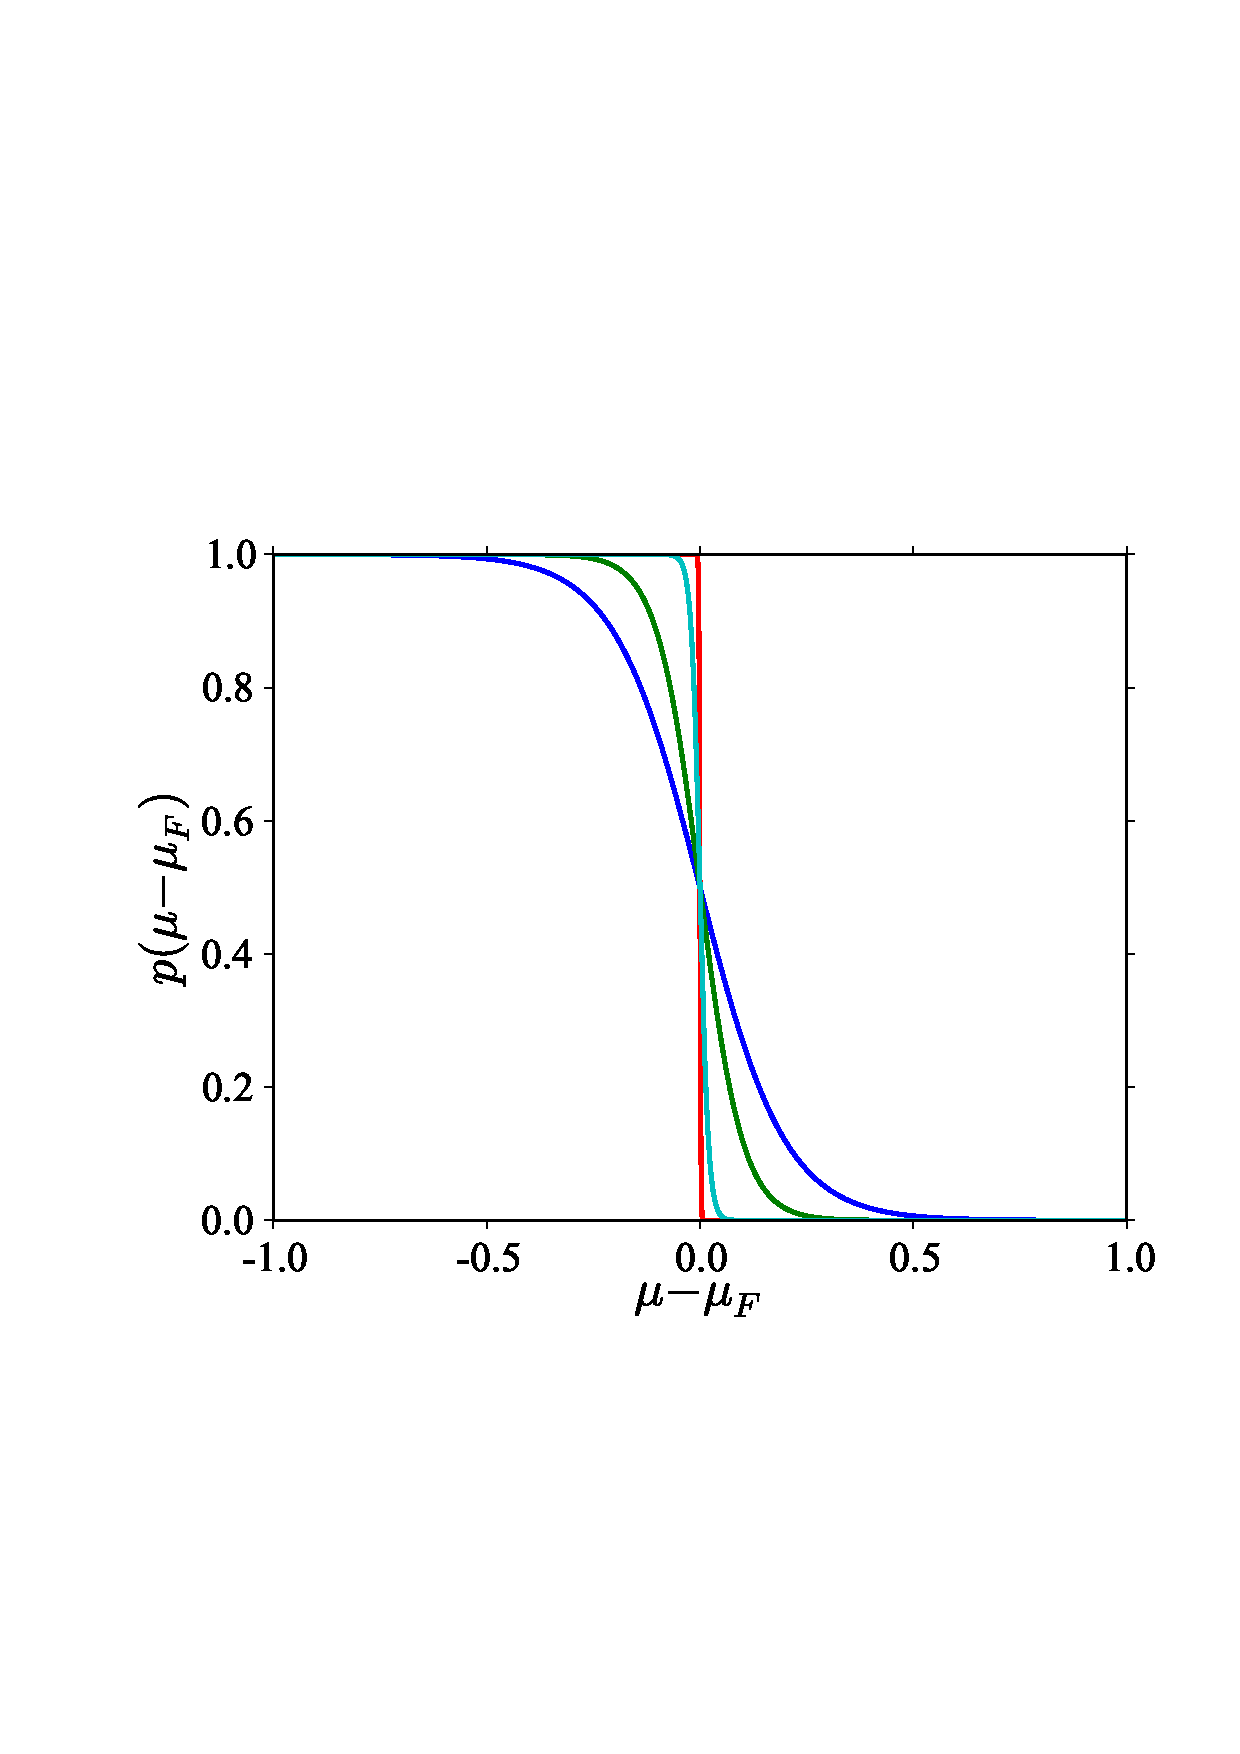
\includegraphics[scale=0.5]{Theorie/Transport/figure2/figure2.pdf} 
\caption{Probabilité d'avoir un électron de potentiel chimique $\mu$ sachant que le potentiel chimique du métal est $\mu_{\rm{F}}$. Le potentiel chimique $\mu_{\rm{F}}$ correspondant à une tension de $1mV$ que l'on applique habituellement dans ce genre d'éxpérience correspond à une énergie de $11.5K$.}
\label{distrib_fermi}
\end{figure}



\subsection{Le potentiel chimique de l'il\^ot}
Si l'expression du potentiel chimique de la source et du drain n'a rien de compliqué (dans le cas d'életrode normale tout du moins), on ne peut pas en dire de m\^eme de celle de l'il\^ot. C'est m\^eme là que réside toute la difficulté de la compréhension d'une expérience. Heureusement, dans la partie précédente nous avons déjà fait le bilan des différentes énergie en jeux dans le système. A savoir, nous devons prendre en compte l'énergie électrostatique du système, l'énergie d'interaction électron-électron ainsi que la discrétisation des niveaux d'énergie dans l'il\^ot. Tout ceci donne :
\begin{eqnarray}
U(N) = \underbrace{\frac{1}{2C_{\Sigma}} (-|e|N + C_sV_s + C_dV_d + C_gV_g)^2}_{\text{couplage électrostatique et énergie de charge}}
+ 
\underbrace{\sum_{n=1}^{N} E_n}_{\substack{\text{énergie liés aux} \\\text{aux états discret}}}
\end{eqnarray}
On peut également tenir compte d'un éventuel champ magnétique en faisant le remplacement suivant :
\begin{eqnarray}
\sum_{n=1}^N E_n = \sum_{n=1}^N E_n(B) \nonumber
\end{eqnarray}
c'est à dire en attribuant à chaque niveau discret, une dépendance en champ magnétique. Nous verrons rapidement dans la suite comment cela se traduit dans le cas d'un système simple. 

Une fois l'énergie en fonction de $N$ exprimée simplement, il suffit d'appliquer la définition précédente à savoir :
\begin{eqnarray}
\mu(N) = U(N) - U(N-1) \nonumber
\end{eqnarray}
On se retrouve avec une expression relativement simple du potentiel chimique :
\begin{eqnarray}
\mu(N) = (N-\frac{1}{2})\frac{e^2}{C_{\Sigma}}
+ 
\frac{e}{C_{\Sigma}}(C_gV_g + C_sV_s + C_dV_d)
+
E_N(B)
\end{eqnarray}

En utilisant la définition de l'énergie de charge $E_c$ introduite précédemment, nous pouvons réécrire la relation sous la forme :

\begin{eqnarray}
\mu(N) = (N-\frac{1}{2})E_c
- 
\frac{E_c}{|e|}(C_gV_g + C_sV_s + C_dV_d)
+
E_N(B)
\label{pot_chim}
\end{eqnarray}

L'énergie $E_c$ est donc la quantité d'énergie d\^u à la répulsion Coulombienne qui sépare deux potentiels chimiques d'état de charge différents.


\section{Détermination des conditions de circulation d'un courant}
Pour rendre l'exposé qui va suivre plus clair, nous allons le décomposé en trois partie. Dans la première partie, nous allons voir quelles sont les conditions à remplir pour qu'un électron du drain puisse aller dans l'il\^ot. Dans la deuxième partie, nous ferrons de m\^eme pour la source. Enfin, dans la dernière partie, nous exploiterons les résultats obtenues pour en déduire les conditions nécessaire pour qu'un courant circule dans notre structure ainsi que le signe de ce courant en fonction des paramètres. Afin d'adapter les solutions trouvées au condition expérimentale, on posera $V_s = 0$ car dans la grande majorité des dispositif, une des électrodes est directement connecter à la masse. Ce qui donnera $V_d=V_{ds}$, $V_{ds}$ étant la tension appliqué à l'échantillon au traver de la source et du drain.

\subsection{Charge de l'il\^ot par le drain}
Comme nous en avons discuté précédemment, pour qu'un particule (ici un électron) puisse passer d'un réservoir à l'autre, il faut que son potentiel chimique soit identique dans les deux réservoirs. Si l'on adapte se raisonnement à notre système, il faut donc qu'il y ait dans le drain des électrons dont le potentiel chimique corresponde à celui de cette électron une fois sur l'il\^ot. Supposons l'il\^ot dans l'état de charge $N-1$, pour passer à l'état de charge $N$, il faut qu'il y ait au moins un électron dans le drain dont le potentiel chimique soit égale à $\mu(N)$. Il nous suffit d'oberver la courbe de la Fig. \ref{distrib_fermi} pour comprendre que cela suppose :
\begin{eqnarray}
-|e|V_{ds} \geq \mu(N) \nonumber
\end{eqnarray}
Ce qui conduit à la relation suivante :
\begin{eqnarray}
-|e|V_{ds} \geq (N-\frac{1}{2})\frac{e^2}{C_{\Sigma}}
-
\frac{|e|}{C_{\Sigma}}(C_gV_g + C_sV_s + C_dV_d)
+
E_N(B) \nonumber
\end{eqnarray}
Puis, en se rappelant que $V_s= 0$ et que $V_{ds} = V_d$ :
\begin{eqnarray}
V_{ds} \leq \frac{1}{C_{\Sigma}}(C_gV_g + C_dV_{ds}) + \frac{E_N(B)}{|e|} - (N-\frac{1}{2})\frac{|e|}{C_{\Sigma}} \nonumber
\end{eqnarray}
Cette relation peut se réécrire de la façon suivante :
\begin{eqnarray}
V_{ds} \leq \frac{1}{C_g + C_s} \{C_gV_g - \frac{C_{\Sigma}}{|e|}[E_N(B) + (N-\frac{1}{2})E_c] \}
\end{eqnarray}

La zone de transition entre charge et décharge dans le plan ($V_g$,$V_{ds}$) est délimité par une droite dont la pente est donnée par les différentes capacitances du système. Cette pente est donnée par 
\begin{eqnarray}
\frac{C_g}{C_g + C_s} \nonumber
\end{eqnarray}



\begin{figure}
\includegraphics[scale=0.5]{Theorie/Transport/figure3/figure3.pdf} 
\caption{Représentation de la charge et de la décharge de l'il\^ot dans le plan ($V_g$,$V_{ds}$)}
\label{charge_discharge}
\end{figure}



\subsection{Charge de l'il\^ot par la source}
Un raisonnement similaire au précédent et en se rappelant que $V_s = 0$ conduit à la relation suivante :

\begin{eqnarray}
V_{ds} \geq -\frac{1}{C_d} \{C_gV_g + \frac{C_{\Sigma}}{|e|}[E_N(B) + (N-\frac{1}{2})E_c] \}
\end{eqnarray}


On peut extraire une deuxième pente qui correspond à la charge ou la décharge de l'il\^ot par la source :
\begin{eqnarray}
-\frac{C_g}{C_d} \nonumber
\end{eqnarray}


De plus nous pouvons en déduire une deuxième relations importantes. Deux états de charge consécutifs sont séparé par une tension de grille $\Delta V_g$ que l'on peut relier aux paramètres du système par la formule suivante:
\begin{eqnarray}
\frac{C_g}{C_{\Sigma}} |e| \Delta V_g = E_c + \Delta E
\end{eqnarray}

\subsection{Condition de circulation du courant}

Si l'on reprend les deux paragraphes précédent, on peut imaginer quatre situtations :
\begin{itemize}
\item \textbf{Situation 1} : aucun électron ne peut \^etre chargé ni par la source ni par le drain. L'état de charge reste à N.
\item \textbf{Situation 2} : un électron peut \^etre chargé à la fois par la source et par le drain. Il va donc y demerer et l'état de charge est N+1.
\item \textbf{Situation 3} : un électron ne peut \^etre charge que par la source. Dans ce cas, il finit par se décharger dans le drain
\item \textbf{Situation 4} : un électron ne peut \^etre chargé que par le drain. Dans ce cas, il finit par se décharger dans la source. \newline
\end{itemize}

Dans les situations un et deux, l'état de charge de l'il\^ot est bien défini et on se trouve dans le régime de blocage de Coulomb. Dans la situation 3 les électrons circulent de la source vers le drain. Un courant positif est donc mesuré. Dans la situation 4, les électrons circulent du drain vers la source. Un courant négatif est donc mesuré. L'emsemble de ces régimes est représenté dans la Fig. \ref{charge_discharge}.

\section{Etats excités et transport}
Dans ce dernier paragraphe nous allons aborder la notion de spectroscopie par transport. Cette méthode vise à analyser les différents état du système par des mesures de transport. Cette technique à notablement été utilisé pour sonder les niveaux magnétique par l'application d'un champ et par l'étude de l'évolution des propriété de transport en fonction de ce champ magnétique.

Nous allons pour aborder cette technique, nous consacrer sur le système que nous avons décrit précédemment dans le cadre de l'équation pilote. Le diagramme Zeeman de l'état de charge N=1 est représenté avec les potentiels chimique associé à la transition 0/1.

A partir de ces potentiels chimique on peut déjà esquissé l'allure de la cartographie de conductance dans le plan ($V_g$,$V_{ds}$). Il suffit pour cela de tracer un double jeux de Diamant de Coulomb. On utilise ensuite les bord de Diamant correspondant à la transition état fondamental de l'état 0 à l'état fondamental de l'état de charge 1. Lorsque d'un bord de Diamant associé à un état excité, ce bord de Diamant doit \^etre stoppé et ne pas allé jusqu'à l'origine. On peut identifier deux zones de lecture pour ce qui est des états d'énergie : par la tension de grille en prolongeant les bords de diamant de Coulomb ou par la tension source drain. Dans les deux cas, une renormalisation de l'énergie est nécessaire.

Une approche plus qualitative peut \^etre obtenue en utilisant les équations pilotes et confirme ce que l'on avait obtenue avec la méthode plus simple des potentiels chimique. En revanche, la technique de l'équation pilote nous donne plus d'information sur l'amplitude des différentes variations de courants.

Ces deux marche successive en courant correspondent à l'entré dans la fen\^etre de tension $V_{ds}$ d'un puis de deux canaux correspondant respectivement à la transition état fondamental état fondamental et état fondamental excité. Dans des système plus complexe, ils arrivent souvent que les état N/N+1 possèdent tout deux des états fondamentaux et des états excités. Dans ce cas, la signature en transport devient plus complexe. Ces différentes configurations sont notamment traité par Hanson et Al., et un exemple peut \^etre trouvé dans l'analyse du $N@C_{60}$ proposé en fin de thèse et les références qu'il contient.

\begin{figure}
\includegraphics[scale=0.5]{Theorie/Transport/figure4/figure4.pdf} 
\caption{Diagramme Zeeman de l'état de charge N=1. Potentiel chimique correspondant à la transition 0/1}
\label{charge_discharge}
\end{figure}

On peut également une autre mesure qui prendra tout son sens dans la suite quand on utilisera l'il\^ot central non plus comme le système à étudier mais comme un sonde de son environnement local. Nous vennons de voir que la position du point de dégénérescence dépend de la position du potentiel chimique dans l'échelle des énergies. On peut donc choisir une tension de grille $V_g$ proche du point de dégénérescence avec une tension source-drain $V_{ds}$ nulle. On mesure en suite la conductance en faisant varier le champ magnétique.$

\section{Cotunneling}

\section{Effet Kondo}